\documentclass[twoside]{article}
\usepackage{amsmath,amssymb,amsthm,graphicx}
\usepackage{epsfig}
\usepackage[authoryear]{natbib}

\usepackage{geometry}
\usepackage{setspace}
\usepackage{float}

\geometry{twoside,
          letterpaper, % i.e, paperwidth=210mm and paperheight=297mm,
          top=25mm,
          bottom=40mm,
          left=25mm,
          right=25mm,
}

\setlength{\parindent}{0pt}
\setlength{\parskip}{0.5cm plus4mm minus3mm}

\begin{document}

\textbf{Project Progress Report - Bayesian Inference for Switching State Space Models}\\
\textbf{Nicholas Hoernle \hfill \today}

\textbf{Work accomplished so far:}

I have explored some of the Dirichlet process~(DP), hierarchical Dirichlet process~(HDP) and hierarchical Dirichlet process for hidden Markov model~(HDP-HMM) literature \cite{fox2007developing,fox2011bayesian,fox2008hdp,teh2005sharing}. To assist my understanding of the DP, I wrote a generative model of a mixture of 4 Gaussians and I wrote a basic Stan model for inference over the parameters (with a stick breaking prior but a truncated number of components). The implementation marginalizes over the cluster assignments ($z_i$) for compatibility with NUTS and uses the posterior distributions of the parameters to make MLE cluster assignments. The Stan implementation is exceedingly slow but the implementation was useful for my understanding.

I have also implemented a blocked Gibbs sampler for the sticky HDP-HMM, detailed in Algorithm 2 of \cite{fox2007developing} and discussed further in \cite{fox2008hdp}. I ran a test on a small generated time series where sequential data are generated from three Gaussian modes. The sticky HDP-HMM recovers the mode assignments and regime means as is presented in \cite{fox2007developing}. I used a truncation level of $L=15$ modes. I ran the Gibbs sampler for $100$ iterations and I used the final sample as a point estimate for the posterior. Due to the problems of label switching, it is not yet clear to me how to get a mean estimate of the cluster assignments from many samples (the sampler appears to switch among some subset of `active' labels). It was interesting to investigate the effect of the `sticky' parameter that encourages self transitions in the HMM. Figure~\ref{fig:sticky_hmm_outputs} shows that the HDP-HMM without the sticky parameter ($\kappa = 0$) finds a noisier mode sequence with more mode transitions and more possible modes than the HDP-HMM with a high sticky parameter ($\kappa = 100$).

\begin{figure}[H]
\centering
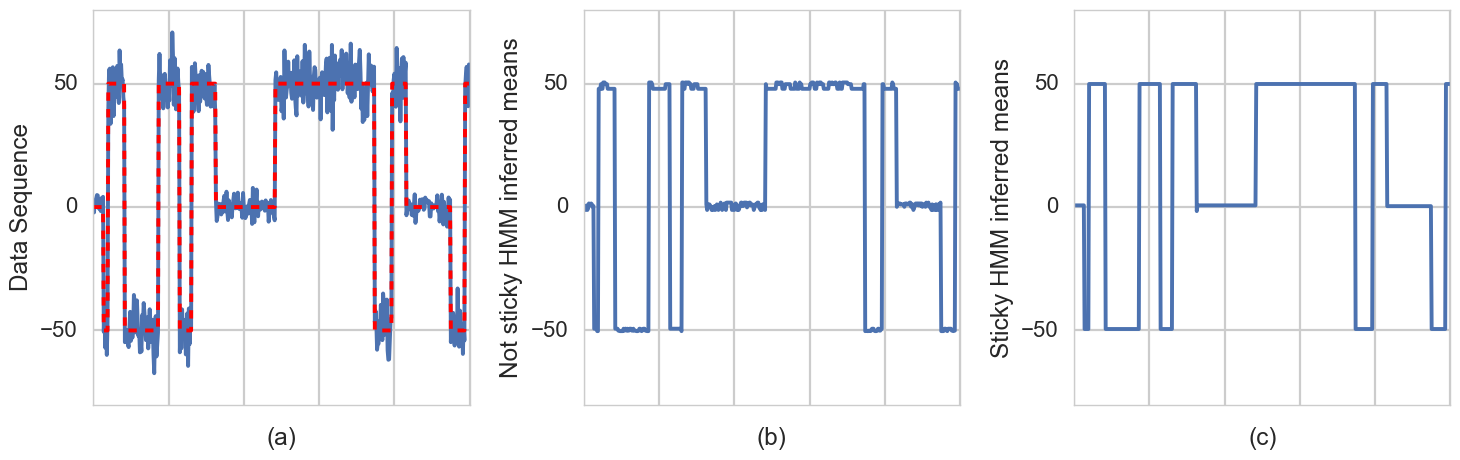
\includegraphics[width=14cm]{sticky_hmm_outputs.png}
\caption{(a) generated data sequence - there are $3$ true modes. Right two plots show the inferred means and mode assignments with (b) $\kappa=0$ (model infers $15$ modes) and (c) $\kappa=100$ (model infers $5$ modes).}
\label{fig:sticky_hmm_outputs}
\end{figure}

\textbf{Plan for rest of project:}

The rest of the project aims to implement the Gibbs samplers for the HDP-SLDS and HDP-AR-HMM models from \cite{fox2011bayesian}. I will begin by implementing and reproducing the tests on generated data for the HDP-AR-HMM model. If time permits, I will expand this implementation to that for the HDP-SLDS.
\begin{enumerate}
  \item Implement the forward and backward recursions for the state space model in the AR/SLDS models (I have already written HMM filters for the implementation above).
  \item Write the Gibbs sampler that is discussed in \cite{fox2011bayesian} for the HDP-AR-HMM model.
  \item Expand upon (2) to develop the Gibbs sampler for the HDP-SLDS model (if time permits).
  \item Reproduce the tests from \cite{fox2011bayesian} (specifically I'd like to reproduce Figure 2) on a similar generated data set.
\end{enumerate}

\newpage
\bibliographystyle{abbrv}
\bibliography{references}

\end{document}
